\documentclass[a4paper,12pt]{article}
\usepackage[utf8]{inputenc}
\usepackage[ngerman]{babel}
\usepackage{amsmath, amssymb}
\usepackage{graphicx}
\usepackage{float}
\usepackage{geometry}
\usepackage{booktabs}
\geometry{a4paper, margin=1in}

\title{Untersuchung der galaktischen Rotation durch 21 cm-Linienprofile}
\author{Astronomisches Praktikum \\
Sommersemester 2024\\\\
Guilherme Schmid}
\date{}

\begin{document}

\maketitle

\section*{Zielsetzung}
Ziel des Versuches war es, die Rotationsgeschwindigkeiten in der Milchstraße durch die Analyse der 21 cm-Emission von neutralem Wasserstoff (H I) zu untersuchen. Dabei wurden die Geschwindigkeiten in Abhängigkeit von der galaktischen Länge \( l \) vermessen und die Verteilung der H I-Wolken bestimmt.

\section*{Durchführung}
Die Daten wurden anhand von 72 beobachteten Profilen der 21 cm-Linie aufgenommen, die innerhalb der galaktischen Ebene (b =±2°) in Schritten von etwa ∆l = 5° gewonnen wurden. Für die Umrechnung der gemessenen Abstände in Relativgeschwindigkeiten wurde eine Kalibrationsskala verwendet, wobei 200 km/s einer Länge von 24 mm entspricht.

\section*{Auswertung}

\subsection*{Umrechnung der Abstände in Relativgeschwindigkeiten}
Die Abstände der linksseitigen Maxima (0° < l < 180°) und rechtsseitigen Maxima (180° < l < 360°) wurden vermessen und in Geschwindigkeiten umgerechnet. Die Umrechnung erfolgte mithilfe des Kalibrationsfaktors:
\[
\text{Faktor} = \frac{200 \, \text{km/s}}{24 \, \text{mm}} = 8.33 \, \text{km/s/mm}
\]

\subsection*{Berechnung der Winkelgeschwindigkeit \(\omega_1\)}
Mit der korrekten Gleichung 8.2:
\[
v_{\text{rel}} = R_0 \sin l \cdot (\omega_1 - \omega_0)
\]
wurde die Differenz der Winkelgeschwindigkeiten \( \omega_1 - \omega_0 \) berechnet, wobei \( R_0 = 8.5 \, \text{kpc} \) und \( \omega_0 = \frac{220}{8.5} \, \text{km/s/kpc} \) gesetzt wurden. Daraus ergab sich die Winkelgeschwindigkeit \( \omega_1 \).

\subsection*{Bestimmung des Zentrumsabstands \(R_1\)}
Die berechneten Winkelgeschwindigkeiten \( \omega_1 \) wurden genutzt, um die Zentrumsabstände \( R_1 \) der verursachenden Wolken zu bestimmen, basierend auf der galaktischen Rotationskurve.

\subsection*{Darstellung in kartesischen Koordinaten}
Die ermittelten Zentrumsabstände \( R_1 \) wurden skaliert, sodass SZ = 10 kpc entspricht. Die Positionen der H I-Wolken wurden in ein kartesisches Koordinatensystem umgerechnet, wobei die Sonne (S) im Ursprung liegt:
\[
r = R_0 \cos l + \sqrt{R_1^2 - R_0^2 \sin^2 l}
\]
\[
x = r \cos(l + 90^\circ), \quad y = r \sin(l + 90^\circ)
\]

\begin{figure}[H]
    \centering
    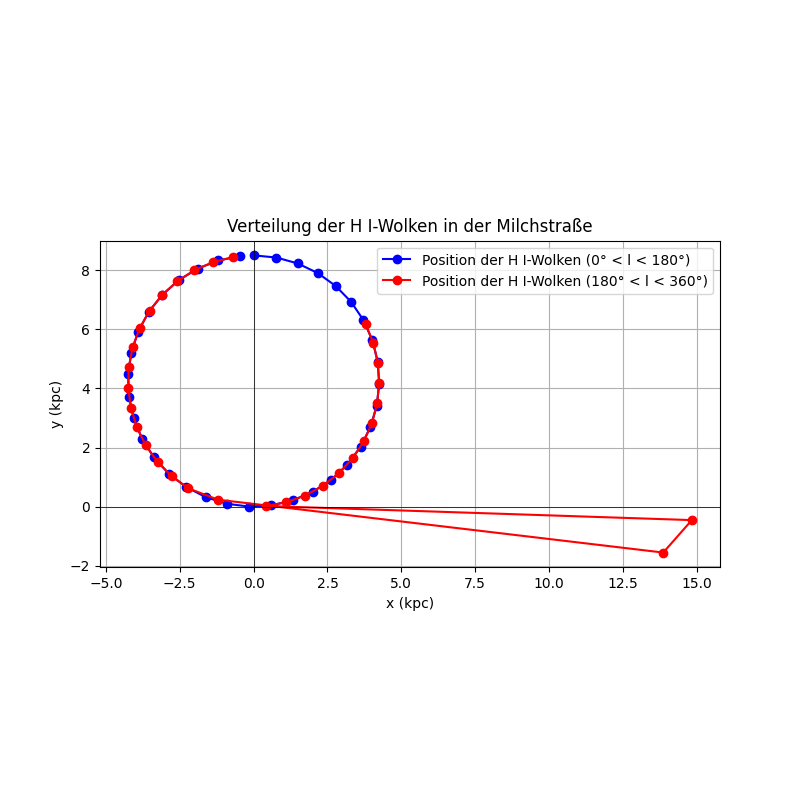
\includegraphics[width=0.8\textwidth]{galatic_h1_distribution.png}
    \caption{Verteilung der H I-Wolken in der Milchstraße}
    \label{fig:galactic_h1_distribution}
\end{figure}

\section*{Ergebnisse}
Die berechneten Relativgeschwindigkeiten und Zentrumsabstände führten zu einer kartesischen Darstellung der H I-Wolken in der Milchstraße. Diese Visualisierung zeigt die Struktur der galaktischen Rotation und die Verteilung der Wolken entlang der galaktischen Ebene.

\section*{Fazit}
Die Analyse der 21 cm-Profile ermöglichte die Bestimmung der Rotationsgeschwindigkeiten der Milchstraße. Die Umrechnung in kartesische Koordinaten ergab eine anschauliche Darstellung der galaktischen Struktur, welche die Verteilung der neutralen Wasserstoffwolken entlang der galaktischen Scheibe zeigt.
\section*{Anhang}
Die Berechnungen wurden mit Hilfe eines Python-Skripts durchgeführt, welches die erforderlichen Messdaten und Berechnungen automatisiert hat.




\end{document}

